\section{Switches, cocycles, and boundary separation}\label{sec:10-boundary}

Our goal is to separate every pair of boundary points by a quasiconvex
subgroup, so that the boundary criterion gives a cocompact cubulation
of each filled row. We first extend the central trees and cocycles
across the satellite fans and then the outer fans. The second half
of the section proves that the resulting cocycles supply all the
required separators.

We continue with a terminal vertex row $J=Y_v$ and the filled fan complex of
Section~\ref{sec:09-fans}. Its edge graph is $\mathcal A$ and its acting group
is $\bar J$. In particular, $\mathcal A$ is uniformly hyperbolic, and, for each
individual filling, it is locally finite and the action is proper and
cocompact. Internal and outer apices are denoted by $d$ and $p$, respectively.
All the choices below are made simultaneously over the finitely many row
types. The initial filling depth, and the finite tests required by
Section~\ref{sec:transfer-relative}, may be prescribed in advance.

All chains and cochains in this section have coefficients in $\F_2$.
Occurrences of edges are retained with multiplicity until a pairing is made;
only then do we reduce modulo two. Thus a passage through an apex supplies two
radial half-incidences, even when it uses the same physical edge twice. A
\emph{pure internal} path avoids outer apices and uses true ordinary neighbors
at every internal apex and horizontal midpoint. The boundary word of every
satellite or outer fan has this property. Pair replacements will produce
chains, and these need not be connected.

We use the central trees $W_0$ and their cocycles $\tau_0$ from
Lemmas~\ref{fan:central-trees} and~\ref{fan:central-cochain}. An
\emph{anchor} is a projected panel or slot node of such a tree, and later also
a switch node. In particular, a central radial contribution has a panel
anchor at its apex, whereas a horizontal contribution has a slot anchor at
its midpoint. The angle dictionary of Lemma~\ref{fan:angle-dictionary} and
the marker comparison of Lemma~\ref{fan:marker} will always be used with
bounds fixed before the final filling kernels are chosen. We give the full
order of these choices at the end of the section.

\subsection{Nonmixed panels and the first switches}

At an internal apex $d$, central and satellite incidences can coexist.
Central labels prescribe values on the radial edges of incidence subtrees;
satellite labels must instead integrate cochains around the attached
cycles. We put these two kinds of labels on separate panel vertices.
Thus testing satellite labels at $d$ introduces no central labels there,
and a central panel acquires no satellite attachment at its own apex.
The later separation proofs will still check the contributions transmitted
through other apices.

\begin{definition}\label{boundary:total-panels}
A \emph{side} is a pair $(W_0,a)$ where the central tree $W_0$ has an
anchor occurrence on the boundary of an actual satellite arm $a$ at its
source $d$. The tree retains its system label and,
when copies are taken, its copy index. The side is \emph{odd} if
$\tau_0^{W_0}$ has total one on the indexed boundary cycle of $a$.
Consuming this side means assigning this particular incidence to one
satellite panel and choosing an anchor occurrence on $a$ for its attachment.

A \emph{central-only total panel} is a central panel $b$, with no additional
attachment at $d$. A \emph{satellite-only total panel} $T$ has no central
panel and consumes finitely many odd $W_0$-sides on the satellite arms at
$d$, an even number on each arm. For every consumed side, attach a spoke
from $T$ to its chosen anchor occurrence. The spoke projects to that tagged
satellite radial edge. Its germ at $d$ is required to be far from every
other spoke germ of $T$.

On each satellite arm, the binary labels of $T$ are a primitive of the sum
of the boundary cochains of the sides it consumes there. Such a primitive
exists because the number of odd sides is even. Its additive constant is
chosen independently on each arm. Central labels of $T$ are zero. Empty
satellite-only panels, including their independent constant labels, are
allowed.
\end{definition}

Figure~\ref{fig:fans-nonmixed-panels} shows these two kinds of abstract
panel over one physical apex. The fan spaces themselves were shown in
Figure~\ref{fig:fan-templates}.
\begin{figure}[tbp]
\centering
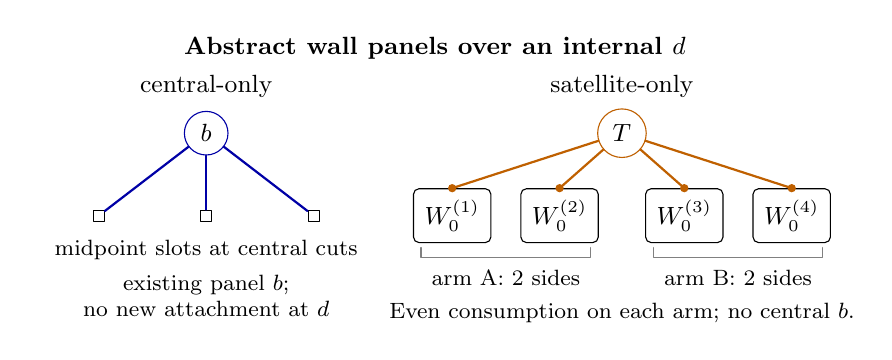
\begin{tikzpicture}[x=.88cm,y=.88cm,font=\small,
  every node/.style={align=center},line cap=round,line join=round,
  apex/.style={circle,draw,fill=white,inner sep=3pt},
  slot/.style={rectangle,draw,fill=white,inner sep=2pt}]
  \node[font=\small\bfseries] at (6,1.8)
    {Abstract wall panels over an internal $d$};
  \node at (2.7,1.24) {central-only};
  \node at (8.7,1.24) {satellite-only};
  \node[apex,draw=blue!65!black] (bc) at (2.7,.57) {$b$};
  \node[apex,draw=orange!75!black] (ts) at (8.7,.57) {$T$};
  \foreach \x/\name in {1.15/c1,2.7/c2,4.25/c3} {
    \node[slot] (\name) at (\x,-.62) {};
    \draw[thick,blue!65!black] (bc)--(\name);
  }
  \node[font=\footnotesize] at (2.7,-1.12) {midpoint slots at central cuts};
  \node[font=\footnotesize,text width=4.3cm] at (2.7,-1.78)
    {existing panel $b$;\\no new attachment at $d$};
  \foreach \x/\i in {6.25/1,7.8/2,9.6/3,11.15/4} {
    \node[draw,rounded corners=2pt,inner sep=4pt] (w\i)
      at (\x,-.62) {$W_0^{(\i)}$};
    \draw[thick,orange!75!black] (ts)--(w\i.north);
    \fill[orange!75!black] (w\i.north) circle (1.5pt);
  }
  \draw[gray] (5.8,-1.08)--(5.8,-1.22)--(8.25,-1.22)--(8.25,-1.08);
  \draw[gray] (9.15,-1.08)--(9.15,-1.22)--(11.6,-1.22)--(11.6,-1.08);
  \node[font=\footnotesize] at (7.025,-1.52) {arm A: $2$ sides};
  \node[font=\footnotesize] at (10.375,-1.52) {arm B: $2$ sides};
  \node[font=\footnotesize] at (8.7,-2.02)
    {Even consumption on each arm; no central $b$.};
\end{tikzpicture}
\caption{Nonmixed panels in the filled complex. The central-only panel
$b$ and satellite-only panel $T$ are abstract wall vertices projecting to
one internal apex $d$. The former joins midpoint slots at its central
cuts. The latter joins chosen anchor occurrences (colored dots) in odd
sides $(W_0,a)$, consuming an even number on each arm; two per arm are
shown only as an example. Across labeled copies, every odd side is
consumed exactly once. A $W_0$-copy may still have sides at other source
apices. Spoke angles are large in the graph metric at the physical image
$d$, irrespective of the drawn Euclidean angles. No additional avoidance
of central cuts is required. A satellite-only panel contains no central
$b$, and its central labels are zero.}
\label{fig:fans-nonmixed-panels}
\end{figure}


\begin{lemma}[Satellite profile tests]\label{boundary:satellite-profiles}
Fix bounds on the number of target ordinary satellite sites and forbidden
germ directions at $d$, and fix an angular avoidance threshold. A finite
pool containing the odd seeds of Proposition~\ref{fan:odd-seeds} supplies
satellite-only panels whose labels realize every binary assignment to a
partition of the target list into classes. Each class lies on one arm and
has bounded cyclic period-coordinate diameter. Their spoke germs avoid the
forbidden directions and one another by the prescribed threshold. The
class-diameter bound and the required filling tests depend only on these
fixed requests and the original finite data.
\end{lemma}

\begin{proof}
On each arm, order the listed sites cyclically. Join consecutive listed
sites into one cluster when the intervening gap is smaller than a fixed
threshold $D$. There are at most as many clusters as targets, and the
diameter of each cluster is at most the number of targets times $D$. A
prescribed binary assignment changes value across an even number of the
cyclically ordered gaps. For each such change, place a translate of an odd
seed with its entire support cluster inside that gap. Its contribution
changes the primitive by one between the neighboring target clusters.

The seed's support has uniformly bounded width. Its chosen anchor rotates
freely, and the angle dictionary bounds the number of rotations whose spoke
lies angularly close to a forbidden direction or a previously placed
spoke. There are only boundedly many directions and earlier placements.
Choose $D$ larger than the support width, the required end margins, and the
number of forbidden positions. Every required placement is then possible.
The additive constant on the arm realizes the value on the first cluster.
If the assignment is constant, no seed is needed. All rotations are by
integral period steps; the fixed elementary word lengths only enlarge the
bounds by fixed factors. These choices involve satellite spokes and the
given forbidden directions; they impose no avoidance condition against
central cuts at $d$.
\end{proof}

\begin{lemma}[Equivariant consumption]\label{boundary:consumption}
After taking finitely many labeled copies of a finite pool of central
systems, every odd side can be consumed exactly once. This can be done
equivariantly, with finitely many decorated panel and edge orbits, while
including all the tests of Lemma~\ref{boundary:satellite-profiles} and any
fixed lower bound on switch angles.
\end{lemma}

\begin{proof}
For each of the finitely many apex types, include the full free
$\bar P_d$-orbits of the stipulated decorated profiles. For the actual
finite links, all requests involving lists of the bounded sizes form a
finite set, so this requires only finitely many profiles. Take $m$ copies of
the entire initial central systems, with trivial action on copy indices.

Consider an arm with even period $n$ and rotation generator $c$. The
requested profiles use any odd side and its translate by $c^{n/2}$ equally
often, because they form full $\bar P_d$-orbits. These two sides are distinct:
the support cluster is nonempty and short compared with $n$. Double the
requested multiplicities and choose $m$ even and larger than all the
resulting consumption counts. Each side then has an even number of unused
copies, equal to the number for its antipode.

Consume the unused copies by antipodal pair panels. The pair's germs have
arbitrarily large angle once the period-coordinate avoidance test is
imposed. An unordered pair may have an order-two stabilizer, but a free
orbit of \emph{decorated} pair panels uses two copies of each side in such a
pair. The even residual multiplicities therefore permit these free orbits;
the offsets of their binary labels are transported with the decorations.
There is no need to choose an offset invariant under an involution that
exchanges the two sides.
More explicitly, write $a=c^{n/2}$ and choose two residual indices $i,j$.
The panel indexed by $g$ attaches to $(gs,i)$ and $(gas,j)$; the panel
indexed by $ga$ attaches to $(gas,i)$ and $(gs,j)$. Thus the free orbit
uses one copy of each chosen index at every side, with no action on the
copy indices themselves.

The stabilizer of an odd side at $d$ is trivial. Indeed, arm exclusivity
forces such a stabilizer to preserve its unique arm, and the short-cluster
argument of Lemma~\ref{fan:arm-exclusivity} excludes a nontrivial arm
rotation. Consequently copy indices can be assigned to all consumptions
equivariantly at each representative apex, then transported to its orbit.
At a fixed $d$, a given $W_0$-piece encounters at most one satellite arm, so it attaches
at most once there. Each central panel in each copy remains its own
central-only total panel.

Assignments at distinct source apices impose separate incidence
conditions. Each labeled $W_0$-copy is a single piece with its
original cochain. An odd side at $d$ is consumed once, and an odd side at a
different source is consumed there as well. These assignments add
edges to that same piece without changing its copy index or its central
cochain. Radial primitives belong to their tagged source arms, so choices
at different sources prescribe values on different radial edges.

Different central systems in the pool retain their tags, slots, and
cochains. Taking their disjoint union does not require rematching slot
data. If satellite tests are not requested in a particular system, the
antipodal construction alone suffices, without an odd-seed hypothesis.
\end{proof}

Let $W_1$ be a component obtained by joining $W_0$-pieces through the
satellite-only total panels. A central-only panel is an existing node,
rather than an additional switch.

\begin{lemma}[The internal trees and their cocycles]\label{boundary:internal-trees}
The $W_1$ are uniformly quasi-isometrically embedded trees, injective on
projected nodes. Each contains at most one total panel over a given internal
apex. They carry equivariant cocycles $\tau_1$ on the internal graph, closed
on all central and satellite fan triangles. A nonzero value on a satellite
radial edge $s\to t$ has one of the following explanations:
\begin{enumerate}[label=\textup{(\roman*)}]
\item $W_1$ contains its total panel at $s$;
\item a constituent $W_0$ has an anchor on that arm within a uniformly
bounded period-coordinate distance from $t$, accessible from $t$ by a short
internal boundary arc.
\end{enumerate}
The bounds, and the quasi-isometry constants, depend only on minimum bend
requirements and the basic central support bounds. Increasing subsequent
angular separations does not increase these constants.
\end{lemma}

\begin{proof}
Use the satellite-only panels as markers in Lemma~\ref{fan:marker}. By arm
exclusivity, a piece attached at $d$ avoids the physical vertex $d$, even at
its internal vertices. Each spoke has length one. Consecutive switches
through a piece are distinct, and their connectors avoid both end markers.
The equivariant consumption construction attaches a piece at most once at
any specified marker. The marker comparison thus gives a tree and the
claimed node uniqueness and uniform embedding. Since every $W_1$-edge
projects to a single graph edge, a reduced path leaving a node does not
revisit its projected vertex.

On the central graph define $\tau_1$ as the sum of the $\tau_0$ of the
constituent copies. For a satellite arm $a$ at $d$, start its radial labels
with those of the satellite-only panel $T$ at $d$, if present, and with zero
otherwise, including the central-only case. For each unconsumed
\emph{even} encounter of a constituent $W_0$, add the primitive of its
boundary cochain on $a$, normalized to zero outside its short support
interval. The complementary long gap makes this normalization unambiguous
for large $n$; a zero boundary cochain receives the zero primitive.

Every odd encounter is already accounted for: its consuming panel belongs
to the same component. A side consumed on a different arm at $d$ has no
support on $a$, by arm exclusivity. Therefore differences of radial labels
equal the full boundary cochain. This is exactly the cocycle equation on
each satellite triangle; the central equations already hold for $\tau_0$.

A default can be nonzero only within the bounded enlargement of its support
cluster, proving (ii). The direct panel labels give (i), regardless of their
additive constants. The same reasoning handles nonordinary boundary sites.
For a fixed edge there are only finitely many possible nearby anchors, by
local finiteness of the filled graph and the finite decorated slots and
links. Node uniqueness prevents infinitely many constituent pieces from
using a fixed such anchor. All sums are thus defined edge by edge. Every
normalization and decoration is transported equivariantly.
\end{proof}

\subsection{Outer switches and boundary sides}

An \emph{outer encounter} is similarly a pair $(W_1,p)$, where the outer
apex $p$ has its single indexed boundary cycle; it is odd when the
$\tau_1$-total on that cycle is one. This indexes the pairing at each
outer apex separately, even if the same $W_1$ encounters other outer fans.

\begin{lemma}[Outer support clusters]\label{boundary:outer-clusters}
For a fixed $W_1$, the nonzero positions of $\tau_1$ on the boundary cycle
of an outer apex $p$ lie in a bounded cyclic period interval. An odd
encounter has trivial stabilizer in the arm rotation group. The interval
bound is independent of later increases in switch angles.
\end{lemma}

\begin{proof}
By Lemma~\ref{boundary:internal-trees}, each nonzero position has an anchor
at uniformly bounded internal distance. Any two such anchors are at
bounded ambient distance by the shortcut through $p$, and hence at bounded
intrinsic distance in $W_1$. This connecting path avoids $p$, as do the short
internal tails to the boundary sites. The angle and period-coordinate
dictionary at $p$ bounds the cyclic distance between any two nonzero
positions. For large cycle order they consequently lie in one short
interval. An odd encounter has a nonempty cluster. A nonidentity subgroup
of the faithful cyclic rotation action cannot preserve a nonempty cluster
of this bounded diameter when the order is sufficiently large. Only the
minimum quasi-isometry and earlier cluster constants were used.
\end{proof}

At each outer apex, pair every odd $W_1$-encounter with its antipodal
translate. They are distinct by Lemma~\ref{boundary:outer-clusters}. Join
them through a pair switch projecting to $p$. Its two spokes are bounded
paths: follow a radial edge to a contributing site and a short internal
path to an anchor. They avoid every outer apex after departure. Choose the
paths by transport from one decorated side; the opposite spoke is the
antipodal translate. Individual sides have trivial stabilizer, whereas an
unordered pair may have an involution exchanging its ends. This is allowed
at a switch. Each $W_1$ attaches at most once at a specified $p$.

\begin{proposition}[Completed trees and cocycles]\label{boundary:completed-trees}
The resulting components $W=W_2$ are uniformly quasi-isometrically embedded
trees. Their $W_1$-nodes and switch nodes have distinct projections within a
component. They carry cocycles $\tau_W$ on the full simply connected fan
complex, supported in a uniform neighborhood of $W$. Under group transport
the only ambiguity in these cocycles is a sum of vertex coboundaries at
outer switches. There are finitely many decorated node and edge orbits.
\end{proposition}

\begin{proof}
The period-coordinate dictionary makes the two germs of every outer switch
as far apart as any prescribed fixed threshold. The $W_1$-pieces avoid
outer apices, and their short attachment paths avoid them except at the
specified end. All hypotheses of the marker comparison hold. This proves
the tree and embedding assertions and shows that changing $W_1$-pieces
forces a geodesic comparison with a large interior turn at an outer apex.
The comparison threshold can be increased without changing the
quasi-isometry constants. No assertion of simplicity is needed on the
interiors of the bounded outer spokes.

On the internal graph, sum the cocycles of the constituent $W_1$-pieces.
At an outer cycle, all odd pieces present in this component belong to its
unique pair switch there, if such a switch exists. Integrate the sum of
the pair's two cochains around the cycle. Its total is zero, so it has a
primitive; choose either additive constant. Integrate every even-only
piece separately, with its primitive zero off its short support cluster,
and add all these primitives to obtain the radial labels.

The difference of successive radial labels is the internal boundary
cochain. Thus every outer triangle has cocycle sum zero. Together with
Lemma~\ref{boundary:internal-trees}, this proves closedness on every face.
Even defaults are supported near anchors; the paired contribution, even
when its primitive is nonzero along a long interval, lies on edges incident
to its switch $p$. Hence the full support is uniformly near $W$. The same
nearby-anchor argument as before proves local finiteness of the sums.

Changing the constant for the paired primitive changes precisely the
values of all radial edges incident to that outer apex. Since that apex
has just its one fan arm, the change is the coboundary of its vertex
indicator. The possible order-two stabilizer of the unordered pair
therefore creates exactly this permitted ambiguity and no further one.
All even normalizations are equivariant.

Finally, the central data, finite links, decorated profiles, and labeled
copies have finite orbit sets. At an outer cycle only finitely many nearby
anchors contribute, so the pair-switch and chosen spoke data also have
finitely many orbits. This proves the last assertion.
\end{proof}

\begin{lemma}[From a cocycle to boundary separation]\label{boundary:sides}
For each $W$, its stabilizer is quasiconvex in $\bar J$ and acts
cocompactly on $W$. The cocycle defines a locally constant binary coloring
on $\partial\bar J\setminus\Lambda W$. Its stabilizer preserves the two
colors up to a global flip. If two points outside $\Lambda W$ have different
colors, a quasiconvex codimension-one subgroup separates them in the sense
of the Bergeron--Wise criterion.
\end{lemma}

\begin{proof}
If two decorated nodes of one component are in the same ambient group
orbit, any group element carrying one to the other preserves their
component. Finiteness of the ambient decorated orbit sets therefore gives
a finite quotient of $W$ by its stabilizer. Node stabilizers are finite,
since the projected action on $\mathcal A$ is proper. The stabilizer acts
properly and cocompactly on the tree, and its orbit embeds
quasi-isometrically in the hyperbolic graph. It is consequently a
quasiconvex subgroup, and its limit set equals $\Lambda W$. Every point of
that limit set is represented by a projected tree ray from any chosen
node.

Simple connectivity lets us integrate $\tau_W$ to a binary vertex coloring,
unique up to one additive constant. A geodesic ray to a point outside
$\Lambda W$ eventually escapes every fixed neighborhood of $W$. It has an
eventual color because the cocycle is supported near $W$. For nearby ideal
endpoints, based rays fellow travel beyond a segment already far from $W$;
short connecting bridges also avoid the support. They have the same
eventual color. This proves both independence of the ray and local
constancy on the complement of the limit set.

Under an element preserving $W$, the cocycle changes by vertex
coboundaries at switch apices. Their primitive is zero away from these
apices. Thus the integrated colors away from the switch set change by one
global bit. On ideal points outside $\Lambda W$ this gives either
preservation or a simultaneous flip. Pass to the kernel of this action on
two colors, of index at most two, and call it $H$. It has the same limit set
and remains quasiconvex.
Concretely, if $\tau_W=\delta f$ and $g$ preserves $W$, write
$g\tau_W+\tau_W=\delta\eta_g$, where $\eta_g$ is supported at its outer
switch vertices. Connectedness gives
\[
 gf+f+\eta_g=\epsilon(g)\qquad(\epsilon(g)\in\F_2).
\]
Off the invariant switch set this is $gf+f=\epsilon(g)$. Composing two
transports there shows that $\epsilon$ is a homomorphism. The possibly
infinite switch set causes no summability problem: $\eta_g$ is a vertex
cochain, and its coboundary is evaluated on one edge at a time.

Choose a fixed neighborhood of an $H$-orbit containing the cocycle support.
Rays of different eventual colors lie in different components of its
complement: any connecting edge path would have zero cocycle sum and hence
preserve the color. Both components are deep, since these rays escape every
fixed orbit neighborhood. Thus $H$ is codimension one. The two locally
constant color classes also show that the given boundary points lie in
different components of $\partial\bar J\setminus\partial H$. This is the
hypothesis of \cite[Theorem~1.4]{BergeronWise2012}, including the case of a
finite subgroup separating an already disconnected boundary.
\end{proof}

\subsection{Comparison paths and satellite tests}

We now prove that finitely many successive systems provide the separators.
There are three geometric cases: a large outer gap; a large internal
turn after bounded outer turns have been replaced; and the remaining
case in which all turns are bounded. In parallel, a comparison around
an outer boundary cycle constructs the odd $W_1$-encounters needed for
the first case. This circle argument uses only the internal trees and
does not assume that the completed outer switches already separate
boundary points.

The two uses have different outputs. A circle comparison starts with one
outer boundary cycle and produces an odd $W_1$-encounter. A line comparison
starts with two ideal endpoints and produces a completed $W_2$ whose
cocycle separates them. Every $W_1$, including those produced by the
circle tests, already has the support bound of
Lemma~\ref{boundary:outer-clusters}. That bound uses only the minimum tree
geometry and is unchanged by stronger test angles. Consequently the
outer-gap threshold $A_p$ can be fixed from this bound and the basic
first-direction comparison before the line tests are chosen; the circle
tests establish existence without changing the bound.

\begin{lemma}[Replacing bounded outer turns]\label{boundary:normalization}
Fix a bound $A_p$ on cyclic period gaps at outer turns of a bi-infinite
geodesic $\gamma$. Replacing these turns by boundary arcs and making the
elementary fan detours produces a pure internal uniform quasigeodesic
$\alpha$. Its constants depend only on $A_p$ and the fixed data.
\begin{enumerate}[label=\textup{(\roman*)}]
\item Each physical vertex occurs a bounded number of times on $\alpha$,
and all its occurrences lie in a bounded parameter interval.
\item If an internal apex $d$ lies on $\gamma$, all new germs at $d$ lie
within bounded angular distance of one of its two original germs
$\nu_-,\nu_+$. When these are sufficiently far apart, each neighborhood
contains an odd number of the new radial half-incidences.
\item If all original internal turns have bounded angle, then the angular
diameter of all germs at all visits to any one internal apex on $\alpha$
is bounded.
\end{enumerate}
\end{lemma}

\begin{proof}
A period gap of at most $A_p$ gives a boundary arc of bounded elementary
length; the conversion factor is the maximum of the fixed word lengths.
Detour every satellite radial ending at an apex or midpoint through a
neighboring ordinary site on that arm, and every central radial ending at
a midpoint through a true ordinary endpoint. Fan triangles realize all
these replacements. Their lengths and displacement are bounded, so the
result is a uniform quasigeodesic with the same ideal endpoints. A
quasigeodesic can revisit a vertex only within bounded parameter distance,
which proves (i).

An elementary radial detour changes its germ at $d$ by a bounded avoiding
path. If a replaced outer arc visits a given original $d$, its parent
outer apex is adjacent to $d$. Since both vertices occur on the original
geodesic, they were consecutive there. The inserted directions are close
via that parent apex, and the replacement polygon changes the number of
half-incidences on that side by an even number. This proves (ii).

For (iii), a new internal passage in an inserted arc has a short avoiding
comparison through the parent outer apex. All individual turns are
therefore bounded. Between consecutive visits to an internal apex, the
subpath avoids that apex and has bounded length by (i). It bounds the
angle between the corresponding visit germs, proving the assertion about
cumulative diameter. Arguments excluding outer switches require only
avoidance of outer apices, and do not need (iii).
\end{proof}

There will be two comparison settings. In the \emph{line setting},
$\alpha$ is as in Lemma~\ref{boundary:normalization}, and the tested trees
are the final $W_2$. In the \emph{circle setting}, $\alpha$ is the specified
pure internal boundary path of one outer apex $p$, and the tested trees are
$W_1$. The angle dictionary at $p$ bounds the number and cyclic-coordinate
diameter of visits to any physical site or internal apex. Directions at
such an apex are close via $p$. No ideal-endpoint assertion is used in the
circle setting.

When every test is even, we will pair radial occurrences and replace each
pair by a short boundary path. The replacement is a sum of fan-triangle
boundaries, so it preserves cocycle evaluation. It may disconnect the
chain. The invariant that keeps the final horizontal chain nonzero is
mod-two winding in the circle setting, and mod-two crossing from one end
to the other in the line setting. We verify these invariants in
Lemma~\ref{boundary:horizontal-parity}.

\begin{lemma}[Satellite tests and uncontaminated evaluations]\label{boundary:satellite-test}
At an internal apex $d$ visited by $\alpha$, apply
Lemma~\ref{boundary:satellite-profiles} to its satellite radial site list,
with spoke germs far from every $d$-direction of $\alpha$. The resulting
tree through $T$ evaluates on $\alpha$ exactly as the prescribed satellite
labels on that list. In the line setting its limit set avoids both ideal
endpoints. If all such evaluations are even, the satellite radial
half-incidences can be paired within their classes and replaced by bounded
purely central boundary arcs avoiding $d$.
\end{lemma}

\begin{proof}
First consider comparisons from $d$ to other anchors or ideal endpoints.
In the line setting they avoid every outer apex. Choose the outer switch
turns above the marker-comparison threshold for these paths. Such a
comparison forbids any change of $W_1$-piece through an outer switch, even
on a ray to an ideal endpoint. Thus we may work in the $W_1$ through $T$.

If another anchor $w\ne d$ lay on $\alpha$, compare the tree path to it
with the subpath starting at the last $d$-visit before $w$. This subpath
avoids $d$ after departure and begins with a listed direction. The tree
path is uniformly quasigeodesic, never revisits $d$, and begins with one
of the forbidden, far-away spoke germs. The first-direction comparison
in Lemma~\ref{fan:marker} gives a contradiction. In the circle setting use
the bounded shortcut through $p$; its direction at $d$ is close to the
listed directions through an ordinary neighbor. The identical comparison
with a tree ray excludes either ideal endpoint in the line setting.

It remains to check defaults rather than only exact anchors. A default at
a satellite radial site of $d$ needs an anchor reached along a short arc
of that same arm, avoiding $d$. Appending this arc to the comparison again
contradicts its first direction. For a satellite traversal at $s\ne d$,
a default needs a $W_0$-anchor $w$ on that arm. If $w\ne d$, compare along
$\alpha$ to $s$ and append its direct spoke to $w$, starting after the last
$d$-visit. If $w=d$, the default would require a central $W_0$-node over
$d$. There is none: $T$ is satellite-only, and node uniqueness excludes a
second node with that projection, also across $W_1$-pieces of $W_2$.
Direct labels at $s\ne d$ and horizontal or central contributions require
exact anchors already excluded. Hence only the intended satellite labels
remain.

If every class has even occurrence count, pair its half-incidences. Two
sites in a class lie on one arm at bounded cyclic distance, so replace the
pair of radials by the intervening bounded boundary arc. These satellite
boundaries are pure central paths and avoid their source $d$. The fan
triangles show that the replacement preserves every cocycle evaluation.
Write $B_s$ for a common elementary length bound. It depends on the
comparison-path and list bounds, but not on a subsequently chosen
large-internal-turn threshold.

For infinite chains this is first a local chain identity. Whenever it is
used for a particular separating tree, we have already excluded that
tree's limit set at both ends. Its support then misses the tails and all
bounded-parameter replacement patches there, so only finitely many patches
affect the evaluation. This justifies the infinite-chain version without
an infinite parity sum.
\end{proof}

\subsection{Large internal turns}

\begin{lemma}\label{boundary:large-internal}
In the line setting, a sufficiently large original internal turn of
$\gamma$ is separated by one of the constructed trees. The required turn
threshold $A_d$ is chosen after the satellite replacement bound $B_s$ and
before the regular-case tests below.
\end{lemma}

\begin{proof}
Let $d$ have original germs $\nu_-,\nu_+$ whose angle exceeds $A_d$.
Perform the satellite tests only at this $d$. If a test is odd, the
preceding lemma already gives separation. Otherwise pair and replace the
satellite half-incidences there to obtain $\alpha'$. They all have $d$ as
source and true ordinary sites as targets. Choose $A_d$ larger than the
angle bound supplied by a $B_s$-arc and the germ neighborhoods of
Lemma~\ref{boundary:normalization}. No pair can join the two sides, and no
replacement arc passes through $d$. The remaining central radial counts
are therefore odd near each $\nu_\pm$.

Choose a central-only panel $b$ whose labels are zero and one,
respectively, on \emph{all} central ordinary germs in sufficiently large
fixed angular neighborhoods of $\nu_-$ and $\nu_+$. Require its cuts to
be far from both directions. These neighborhoods contain boundedly many
germs by the angle dictionary. The central panel tests of
Proposition~\ref{fan:central-panels} give the required labels: after their
class-diameter bound is fixed, enlarge $A_d$ so that no class meets both
neighborhoods. A class meeting both would give a bounded horizontal path
avoiding $d$, contradicting that enlarged angle bound.

We claim that every first direction in the $W_1$ of $b$ towards another
node is far from both $\nu_\pm$, with any prescribed fixed comparison
margin. Central edges are controlled by the cuts. The additional
possibility is a spoke from $b$ to a satellite-only panel at another apex
$s$, because the $W_0$ of $b$ has odd total on an arm at $s$ visiting $d$.
Suppose its germ $d\to s$ were close to a $\nu$. An additional anchor
$w\ne d$ on that arm would contradict the first cut from $b$ in $W_0$,
using the shortcut through $s$. Thus this $W_0$ has anchors on the arm only
at $d$. Every central passage at $d$ on that arm has its two neighboring
ordinary germs close to the same direction through $s$. Both receive the
same label, so the passage contributes zero. There are no other
contributions. The total on that arm is even, contrary to the supposed
attachment. This proves the claim; it is the reason for using nonmixed
panels.

Compare from the last $d$-visit along $\alpha$ towards either ideal
endpoint. Outer changes are forbidden by avoidance of outer apices, and
the claim forbids the first direction of the $W_1$-ray. Neither endpoint
belongs to the limit set of the resulting $W_2$.

We check every possible extra contribution on $\alpha'$. An exact anchor
$w\ne d$ on an unchanged portion is excluded by comparison along
$\alpha$. On an inserted arc, use its short tail from a paired $d$-target;
this also avoids $d$ after departure. These comparisons forbid outer
changes and then contradict the first-direction claim.

A satellite half remaining at $s$ has $s\ne d$ and comes from
$\alpha$. Its default requires an anchor $w$ on that arm. The case
$w\ne d$ is excluded through $s$ as before. If $w=d$, node uniqueness
makes the original $W_0$ of $b$ the only possible contributor. Here $s$ is
adjacent to $d$, and the quasigeodesic subpath from the last relevant
$d$-visit to $s$ is bounded. Its first direction, and hence the spoke
$d\to s$, is close to one of $\nu_\pm$. The preceding arm argument
shows that this $W_0$ encounters the arm only at $d$ and has zero sum
between consecutive true ordinary sites. Individual halves of a central
passage need not be zero, but their pair is zero. Its even integration
default is consequently constant on all true ordinary sites. The
short-cluster normalization sets it to zero at distant ordinary sites,
and therefore at every ordinary site. This remaining contamination also
vanishes.

Only the intended central labels at $d$ survive. Their total is one,
since the counts near both original germs are odd and the two labels are
zero and one. Triangle consistency transfers this total to $\gamma$.
All bounds used in excluding the extra contributions depend on the
already fixed substitution, quasigeodesic, and basic cluster constants.
They do not depend on the size of the original large turn.
\end{proof}

\subsection{Regular comparisons and the last horizontal chain}

We next treat both the circle setting and the line setting in which every
original internal turn is at most $A_d$. Apply the satellite tests at every
internal apex met by $\alpha$. If none is odd, make all the paired
replacements, obtaining a pure central chain $\alpha^1$. In the line
setting, the quasigeodesic parameter localizes every pairing to a bounded
interval. In the circle setting, the period-coordinate dictionary gives
the same conclusion in the cyclic parameter.

\begin{lemma}[Regular comparison paths]\label{boundary:regular-comparisons}
Sites participating in $\alpha^1$ have bounded connectors to true ordinary
sites of $\alpha$. Comparisons between them have uniformly bounded
cumulative germ diameter at every internal apex. In the line setting,
they avoid outer apices, are uniform quasigeodesics, and extend to either
ideal endpoint. The lists needed at any tested internal apex have bounded
size. These assertions persist after adding any fixed bounded horizontal
tails to the connectors.
\end{lemma}

\begin{proof}
For a site on an inserted arc, follow that arc to a paired endpoint. Each
internal apex passage on this connector has a short angular bypass through
the arm's source apex, which differs from the apex being traversed. For an
untouched half, use that half to an ordinary neighbor when needed. From a
tested apex, its connector can start with the particular germ being tested.

Join two such tails by the intervening $\alpha$-path in the line setting.
This is a uniform quasigeodesic with bounded end modifications, avoids
outer apices, and extends in the same way towards an ideal end. In the
circle setting join the ordinary ends of the tails by their two spokes
through the parent outer apex $p$, giving a uniformly bounded comparison.
All junctions between the portions are ordinary vertices. Every internal
passage has bounded angle. Repeated visits to any internal apex have
bounded number and bounded intervening lengths, using quasigeodesicity in
the line setting and the bounded comparison length in the circle setting.
Consequently the cumulative angular diameter is bounded, including when a
comparison revisits its initial tested apex: its last germ there remains
close to its prescribed initial one.

Finally, each substitution arc has bounded length and stays close to its
assigned old positions. In the line setting quasigeodesicity bounds all
possible positions assigned to one physical site or apex. In the circle
setting the connector tails avoid $p$, so the angle dictionary at $p$
bounds their cyclic-coordinate ambiguity. These observations also bound
the number of occurrences in each tested list. Extra bounded horizontal
tails change only the bounds and create no new internal turns.
\end{proof}

\begin{lemma}[Central tests on the regular chain]\label{boundary:central-test}
At an internal apex $s$ with radial halves in $\alpha^1$, central panel
tests evaluate exactly the class parities of their ordinary target sites.
An odd test separates the ideal endpoints in the line setting and gives
an odd $W_1$-total on the outer cycle in the circle setting. Otherwise all
remaining radial halves can be paired and replaced by bounded horizontal
link paths, giving a purely horizontal chain $\alpha^2$.
\end{lemma}

\begin{proof}
Use a second central system, with satellite switch bends chosen after the
regular comparison bounds of Lemma~\ref{boundary:regular-comparisons}.
At $s$, distinguish bounded intrinsic classes of the target list and put
the central cuts far from its germ directions.

Every contribution on the pure central chain requires an actual
$W_0$-anchor: either its midpoint or its central apex. A comparison from
the tested panel to such an anchor cannot cross an outer switch in the
line setting, since the comparison avoids outer apices. It cannot change
$W_0$-piece through a satellite switch in either setting, since that would
force an interior turn exceeding the cumulative angular bound on the
comparison. Within the one $W_0$, its first cut excludes every other
anchor. This remains true if the comparison revisits the tested apex,
because its last germ is still close to the initially prescribed one.
Only the target central labels therefore contribute.

A tree ray asymptotic to either ideal endpoint is excluded in precisely
the same order: it cannot use an outer switch, cannot use a satellite
switch, and cannot use a first cut. Thus an odd evaluation gives the
claimed separation. In the circle setting it gives the required odd total
without any endpoint assertion.

If all tests are even, each bounded intrinsic class has even occurrence
count. Pair within these classes and replace the radial pairs by bounded
horizontal link paths. Fan triangles preserve every cocycle evaluation.
Let $B_h$ be a common bound for these new paths. The connectors of
Lemma~\ref{boundary:regular-comparisons} merely acquire horizontal tails
of length at most $B_h$. Pairing at an apex again takes place within a
bounded parameter interval, by its proximity through the previous
connectors to the old comparison path.
\end{proof}

\begin{lemma}[A surviving horizontal edge]\label{boundary:horizontal-parity}
The chain $\alpha^2$ contains a physical horizontal edge with odd
multiplicity. A final central system whose cut and switch thresholds
exceed the new regular comparison bounds has a slot tree with odd total
on this chain. In the line setting its limit set avoids both ideal
endpoints.
\end{lemma}

\begin{proof}
First choose the final system with its central cut separations, satellite
switch bends, and, in the line setting, outer switch bends all above the
bounds supplied by the connectors after the horizontal replacements. Two
distinct horizontal midpoint anchors of $\alpha^2$ cannot belong to one
completed tree. A comparison between them forbids switches at either
level. They would therefore lie in one $W_0$; its path between distinct
slots has an internal panel bend, also forbidden by the same comparison.
Likewise a ray asymptotic to a line endpoint can neither switch nor
continue indefinitely inside $W_0$, because it would have such an
interior bend. This proves the limit-set assertion for every tested slot
tree.

We prove nonzero physical parity without assuming that the modified chain
is connected. In the circle setting, assign each participating physical
vertex its position on the original parameter circle, using its occurrence
or the connector to an original site. All ambiguities have bounded cyclic
diameter: the connectors and replacement patches avoid the parent outer
apex $p$, so the angle dictionary applies. Choose a single position for
each physical vertex and send each edge along its short parameter arc.
This is the short-arc construction used in the proof of
Proposition~\ref{fan:odd-seeds}.
Every replacement polygon lies in a bounded parameter interval and has
degree zero for sufficiently large cycle order. The original boundary
cycle has degree one. The final chain therefore has degree one modulo two
and cannot be the zero physical chain.

In the line setting, assign each participating physical vertex a single
real parameter, chosen from its occurrence or connector positions on
$\alpha$. Quasigeodesicity and bounded tails bound the ambiguity. Cut the
parameter line at a generic finite point and give each physical vertex a
single binary sign according to which side its chosen parameter lies on.
For an edge, count one if the endpoint signs differ. Every replacement
loop has even crossing count, because its sign changes telescope modulo
two. Only bounded-parameter loops can meet both signs, so only finitely
many replacements affect this count. The original bi-infinite path has
opposite signs at its two ends and hence odd crossing count. The final
physical chain is consequently nonzero.

At a horizontal midpoint the cycle condition says that its two half-edge
counts agree, in both settings; local finiteness justifies this condition
in the line setting. Thus some full physical horizontal edge has odd
multiplicity. Choose a slot at its midpoint in the final system. On a
purely horizontal chain only marked slots contribute. No other midpoint
of the chain is marked by this tree, as proved above, and node uniqueness
allows just this one slot over the chosen midpoint across all constituent
pieces. The evaluation is therefore odd.

All evaluations pass back through the substitutions by triangle
consistency. In the line setting the previously proved limit avoidance
ensures that the support misses sufficiently distant tails and their
bounded-parameter patches. Thus only finitely many substitutions affect
this particular evaluation, as required.
\end{proof}

\begin{corollary}[Odd outer encounters]\label{boundary:outer-odd-seeds}
A finite pool of $W_1$-systems contains, on the cycle of every outer apex,
at least one $W_1$ with odd total. The pool and all its required bounds can
be fixed before the final filling depth choices.
\end{corollary}

\begin{proof}
Apply the circle setting. An odd satellite test suffices. If none exists,
perform the satellite pairings. An odd central test then suffices. If none
exists, Lemma~\ref{boundary:horizontal-parity} supplies an odd final slot
tree. Only the finitely many successive systems just described are used;
the bounds depend on the fixed initial circular comparisons and the
preceding pairing bounds. This argument uses $W_1$ throughout and does not
assume any separating outer $W_2$ switch.
\end{proof}

\subsection{Large outer turns and completion of separation}

\begin{lemma}\label{boundary:large-outer}
A sufficiently large cyclic period gap at an outer turn of a geodesic
$\gamma$ is separated by one of the completed trees. The gap threshold
$A_p$ depends only on the basic quasi-isometry and support-cluster bounds,
not on later increased switch bends.
\end{lemma}

\begin{proof}
Let $p$ be that outer apex and let the two traversed sites be its entry and
exit sites. Take an odd encounter from
Corollary~\ref{boundary:outer-odd-seeds} and its antipodal partner. Rotate
the pair so that one entire support cluster lies strictly inside the
shorter interval between the entry and exit sites, and its antipode lies
inside the complementary interval. Give both clusters bounded margins
from the endpoints. The two first spoke germs must also avoid the two
geodesic germs by the fixed first-direction comparison bound. Only
boundedly many rotations are forbidden by this angular condition, by the
angle dictionary. A sufficiently large $A_p$, chosen from the cluster
widths, margins, and this forbidden-position bound, permits the placement.

Every tree path or ray from the switch leaves in one of these two
prescribed directions. It is uniformly quasigeodesic and does not revisit
$p$. The first-direction comparison excludes either endpoint of
$\gamma$ from its limit set.

We must also exclude cocycle contributions away from this traversal. A
nonzero contribution on either side of $\gamma$ would provide a tree
anchor other than $p$, either exactly on that side or accessible by a
uniformly bounded path from it avoiding $p$. For internal edges this is
the support rule of Lemma~\ref{boundary:internal-trees}. At another outer
apex, either that switch itself is an anchor or an even default gives a
short path through that other apex and internally to an anchor. Following
the corresponding side of $\gamma$ from $p$ and then this short path
contradicts the same first-direction comparison. Thus no such
contribution exists.

On the traversal through $p$, the paired odd clusters give integrated
difference one, since exactly one lies in the chosen interval. An
additional even-only piece could change this difference only if an
interval endpoint split its short support cluster. Such a split would
supply an anchor accessible from that endpoint by a bounded internal arc
and short tail, already excluded by the first-direction comparison.
The full difference is therefore one. The required avoidance and margins
used only the uniform minimum-threshold geometry and cluster constants.
\end{proof}

\begin{proposition}[Boundary separation]\label{boundary:separation}
There are finitely many systems of completed trees such that every pair of
distinct points of $\partial\bar J$ lies outside the limit set of one of
the trees and has different cocycle colors there.
\end{proposition}

\begin{proof}
Choose a bi-infinite geodesic for the pair. A large outer gap is handled by
Lemma~\ref{boundary:large-outer}. Otherwise normalize it by
Lemma~\ref{boundary:normalization}. A large original internal turn is
handled by Lemma~\ref{boundary:large-internal}. In the remaining case all
original internal turns are bounded. An odd satellite test separates by
Lemma~\ref{boundary:satellite-test}; failing that, an odd central test
separates by Lemma~\ref{boundary:central-test}; failing both,
Lemma~\ref{boundary:horizontal-parity} supplies the final slot separator.
Each lemma proves limit avoidance as well as odd evaluation. The finite
choice of systems and its compatibility with the filling depths are
verified next.
\end{proof}

\subsection{The order of the finite choices}

\begin{lemma}[No circular choice of thresholds]\label{boundary:scale-order}
All systems used above can be chosen from a finite pool by finitely many
original depth, angle, girth, period-order, and avoidance tests. These tests
can be imposed simultaneously with any initial filling-depth request and
the finite-path tests of Section~\ref{sec:transfer-relative}.
\end{lemma}

\begin{proof}
For clarity, an angular comparison bound below is a value of the fixed
bound functions supplied by the full-graph hyperbolicity and angle
dictionary, for already chosen path constants and list sizes. The number
of original germ types is finite. Thus any finite collection of such
requests is a finite collection of original tests, even though the final
links and their periods depend on the eventual filling.

\begin{enumerate}[label=\textup{\arabic*.},leftmargin=*]
\item First impose the minimum central and internal switch bounds needed
for the marker comparison, the bounded polygon tests, and the inner
support clusters. They give uniform quasi-isometry constants for $W_0$
and $W_1$, independent of any subsequent increase in sparseness. The
outer support-cluster bound follows. Impose the minimum outer switch bound
as well, obtaining fixed quasi-isometry constants for $W_2$.

\item These basic constants determine the outer-gap threshold $A_p$ in
Lemma~\ref{boundary:large-outer}. They therefore determine the
quasigeodesic and visit bounds for the normalized path $\alpha$.
Importantly, $A_p$ uses the \emph{basic} first-direction and cluster
bounds; it does not use later regular-comparison bend requirements.
Include the central odd-seed pool from Proposition~\ref{fan:odd-seeds} wherever
satellite profile tests will be needed.

\item Fix the first satellite tests from the bounds for $\alpha$ and,
simultaneously, from the initial circular comparisons. Their target lists,
forbidden directions, and required first-direction margins are now
bounded. Lemma~\ref{boundary:satellite-profiles} gives their class bound,
and hence the replacement bound $B_s$. No bound on a possibly large
original internal turn has been used.

\item Fix the angular neighborhoods and cut-avoidance requests for the
large-internal-turn test, using only the preceding constants and $B_s$.
The central tests then give their intrinsic class-diameter bound. Choose
$A_d$ larger than the resulting bound for a class straddling both
neighborhoods, and larger than the bound for a satellite pair straddling
them. This is the first choice of $A_d$; its value is not an input to the
tests that determined it.

\item Only now use the absence of turns larger than $A_d$ in the regular
line case. Lemma~\ref{boundary:regular-comparisons} gives the new
cumulative angular bounds, also encompassing the circular case. A second
system has internal switch bends above these bounds and central list
tests whose cuts avoid the relevant directions. Its class bound gives
the horizontal replacement bound $B_h$.

\item The extra horizontal tails of length at most $B_h$ give the final
regular comparison bounds. A final central system has all cut separations
and internal switch bends above these bounds. This is a separate system;
its stronger sparsity need not be fed back into the earlier tests.

\item After all these comparison requests have been recorded, choose
outer antipodal switch bends above their maximum wherever needed. This
is possible by the period-coordinate tests and does not alter the fixed
minimum-threshold quasi-isometry constants. In systems without prescribed
satellite labels, consume odd sides by antipodal pairs with the requested
bend bound; no new seed or class test is needed.
\end{enumerate}

The finite systems for the circle setting give the odd outer encounters
before they are used in the large-outer-turn proof. There is no converse
dependence: the circle setting uses only $W_1$ and the bounded shortcut
through its parent outer apex. Its support bounds already came from the
minimum-threshold geometry.

Every placement condition, polygon-lift length, cyclic-index bound,
minimum period order, girth requirement, and excluded transporter list is
now finite and fixed. The kernel construction of
Proposition~\ref{kernel:construction}, including its graph-cover and order
conclusions in Corollary~\ref{kernel:graph-cover} and
Proposition~\ref{kernel:orders}, together with
Section~\ref{fan:scale-order}, imposes these tests before freezing
$H,\ell,\mathbb k,N$. Membership and injectivity tests used in the angle
dictionary are imposed at their corresponding fixed lengths. Taking their
finite union with the prescribed initial filling and finite-path tests
proves the assertion.
\end{proof}

\subsection{Good fillings and the primitive-extension conclusion}

\begin{theorem}[Virtually compact special filled vertices]\label{boundary:filled-vertices}
For the terminal row and peripheral data constructed in
Sections~\ref{sec:07-transfer}--\ref{sec:09-fans}, one can choose the
height-fiber kernels arbitrarily deep, simultaneously satisfying the
finite-path tests, so that every filled vertex group $\bar J$ is
hyperbolic and virtually compact special.
\end{theorem}

\begin{proof}
Hyperbolicity and the proper cocompact fan model are supplied by the row
filling construction. Elementary filled groups are already virtually
compact special. For every other filled row,
Lemma~\ref{boundary:scale-order} makes the wall constructions and
Proposition~\ref{boundary:separation} simultaneous. By
Lemma~\ref{boundary:sides}, each boundary pair is separated by the limit
set of a quasiconvex codimension-one subgroup. The boundary criterion
\cite[Theorem~1.4]{BergeronWise2012} gives a proper cocompact action on a
CAT(0) cube complex. Agol's theorem \cite[Theorem~1.1]{Agol2013} gives a
finite-index subgroup acting specially on that complex. The quotient is
compact because the original action was cocompact and the index is finite.
Thus the conclusion is virtual \emph{compact} specialness.
\end{proof}

\begin{theorem}[Arbitrarily deep good quotients]\label{boundary:good-fillings}
Let $G$ be the hyperbolic torsion-free primitive extension group under
consideration, with the terminal finite malnormal quasiconvex virtually
compact special peripheral family constructed in the preceding sections.
For every prescribed sufficiently deep filling-avoidance request, there
is a filling of this family to a hyperbolic virtually compact special
quotient. Its peripheral images are finite-by-cyclic or finite, are
hyperbolic virtually compact special, and have the inherited relative
peripheral structure and filling conclusions.
\end{theorem}

\begin{proof}
Impose the given initial request together with the finite-path transfer
and the finite tests of Lemma~\ref{boundary:scale-order}. The terminal
transfer, Theorem~\ref{transfer:finite-path-transfer}, gives the finite
quotient splitting; Proposition~\ref{transfer:ambient-qc} gives ambient quasiconvexity
of its edge groups. Its filled vertex groups are hyperbolic virtually compact
special by Theorem~\ref{boundary:filled-vertices}. Deep relative filling
in $G$ gives relative hyperbolicity of the quotient, with the stipulated
finite-by-cyclic or finite peripheral images. These images are hyperbolic,
so the quotient is hyperbolic. They are also virtually compact special:
a finite group is virtually trivial, and a finite-by-cyclic group is
virtually cyclic.

The hyperbolic quasiconvex hierarchy theorem \cite{Wise2021}, applied to
the transferred finite splitting with these vertex groups, makes the
whole quotient virtually compact special. Here the edge groups are
quasiconvex in the ambient quotient, as required by the transfer result;
this is not an inference from arbitrary embeddings of the vertex groups
in right-angled Artin groups. The inherited peripheral and filling
conclusions are exactly those of the deep relative filling and standalone
row constructions. The initial avoidance request was arbitrary.
\end{proof}

\begin{theorem}[Primitive extensions]\label{boundary:primitive-vcs}
Every hyperbolic torsion-free primitive extension group of either of
Linton's two forms specified in the introduction is virtually compact
special.
\end{theorem}

\begin{proof}
For such a group the primitive data of Section~\ref{sec:03-rows} and the
opening reduction establish local indicability,
coherence, a finite aspherical two-dimensional one-relator model, and
acyclicity of its universal-cover chain complex over the rational Linnell
division field. The preceding actual-row, closure, and terminal arguments
construct the finite malnormal quasiconvex virtually compact special
peripheral family. Theorem~\ref{boundary:good-fillings} supplies arbitrarily
deep good quotients with hyperbolic virtually compact special peripheral
images and the inherited filling conclusions. Thus all hypotheses of the
filling criterion, Theorem~\ref{fill:criterion}, hold. That criterion gives
virtual compact specialness of the original group $G$.
\end{proof}
